\documentclass[border=2mm]{standalone} 

\usepackage{graphicx}
\usepackage{siunitx}
\usepackage[siunitx]{circuitikz}

\begin{document} 
	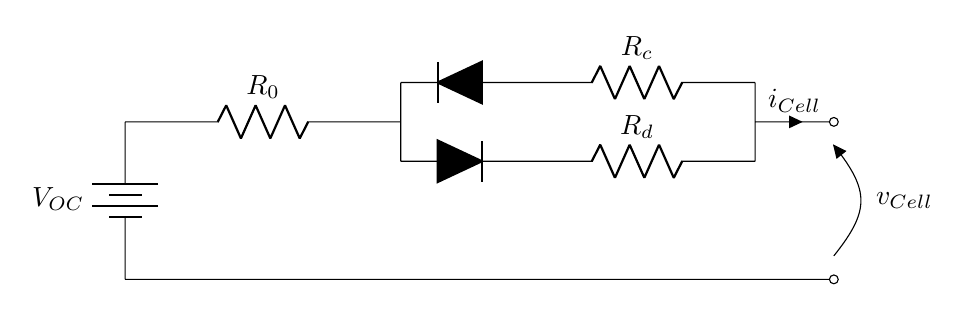
\begin{tikzpicture}[european voltages, american currents]
    
    \ctikzset{voltage/distance from node=10}
    \ctikzset{bipoles/diode/height=.375}

    % Named coordinates
    \coordinate (voc_p) at (0,2);
    \coordinate (voc_n) at (0,0);
    

    \coordinate (left_mid)    at (3.5,2.0);
    \coordinate (left_top)    at ($(left_mid)+(0.0,0.5)$);
    \coordinate (left_bot)    at ($(left_mid)-(0.0,0.5)$);

    \coordinate (right_mid)    at (8.0,2);
    \coordinate (right_top)    at ($(right_mid)+(0.0,0.5)$);
    \coordinate (right_bot)    at ($(right_mid)-(0.0,0.5)$);

    \coordinate (out_p) at ($(right_mid)+(1.0,0.0)$);;
    \coordinate (out_n) at (9.0,0.0);

    \draw
        (voc_p) to[battery, l_=$V_{OC}$] (voc_n)
        (voc_p) to[R=$R_{0}$] (left_mid)


        (left_top) to[short] (left_bot)

        (left_bot) to[D*] ($(left_bot)+(1.5,0.0)$) coordinate (diode_d)
        (diode_d) to[R=$R_d$] (right_bot)

        ($(left_top)+(1.5,0.0)$) coordinate (diode_c) to[D*] (left_top)
        (diode_c) to[R=$R_c$] (right_top)

        (right_top) to[short] (right_bot)


        (right_mid) to[short,-o,i=$i_{Cell}$] (out_p)

        (voc_n) to[short,-o] (out_n)
        (out_n) to[open,v>=$v_{Cell}$] (out_p)
    
        ;\end{tikzpicture}
\end{document}